\documentclass[tikz]{standalone}
\usepackage{pgfplots}
\pgfplotsset{compat=1.15}
\usepackage{mathrsfs}
\usetikzlibrary{arrows,calc}
\usepackage{tkz-euclide}
\pagestyle{empty}
\usepackage{fp}

\definecolor{AngleClr}{rgb}{0,0.39215686274509803,0}
\definecolor{ShapeClr}{rgb}{0.6,0.2,0}

\begin{document}

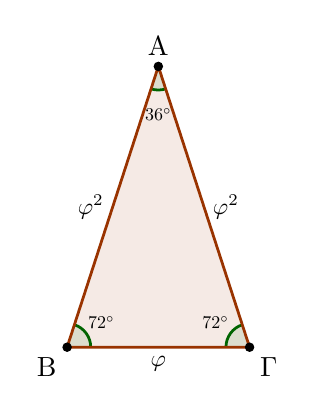
\begin{tikzpicture}[scale=.75]
\tkzSetUpLine[line width=1pt,color=black]
\tkzSetUpPoint[fill=black]

\def\LL{5}
\FPeval{\Xx}{0.3090 * \LL}
\FPeval{\Yy}{0.9510 * \LL}
\FPeval{\R}{2*\Xx}
\tkzDefPoints{-\Xx/0/B,0/\Yy/A,\Xx/0/C}

\tkzFillPolygon[fill=ShapeClr,fill opacity=0.1](A,B,C)
\tkzFillAngles[fill=AngleClr,size=.4,fill opacity=0.1](C,B,A A,C,B B,A,C)
\tkzMarkAngles[line width=1pt,size=.4,color=AngleClr](C,B,A A,C,B B,A,C)

\tkzDrawPolygon[color=ShapeClr](A,B,C)
\tkzDrawPoints[size=3](A,B,C)
\tkzLabelPoint[above](A){$\rm A$}
\tkzLabelPoint[below left](B){$\rm B$}
\tkzLabelPoint[below right](C){$\rm \Gamma$};

\tkzLabelSegment[below,scale=0.85](B,C){$\varphi$}
\tkzLabelSegment[right,scale=0.85](A,C){$\varphi^2$}
\tkzLabelSegment[left,scale=0.85](A,B){$\varphi^2$}

\tkzLabelAngle[pos=1.1,scale=0.65](C,B,A){$72^\circ$}
\tkzLabelAngle[pos=1.1,scale=0.65](A,C,B){$72^\circ$}
\tkzLabelAngle[pos=1.25,scale=0.65](B,A,C){$36^\circ$}

\end{tikzpicture}

\end{document}
